\documentclass[sigconf,review,anonymous]{acmart}
% Accio / SSC paper draft for ICS. Tables in tables/*.tex and figures in figures/*.pdf are generated
% from the Delta results by context-transfer-engine/benchmark/ssc/paper_tables.py; do not edit them
% by hand. \pending{} marks numbers that are still being measured.
\usepackage{booktabs}
\usepackage{xcolor}
\usepackage{listings}
\usepackage{tikz}
\usetikzlibrary{positioning,fit}
\newcommand{\pending}[1]{\textcolor{red}{[#1]}}
\newcommand{\sys}{Accio}
\lstset{basicstyle=\ttfamily\scriptsize,breaklines=true,columns=fullflexible,frame=single,framerule=0.3pt}
\settopmatter{printacmref=false}
\setcopyright{none}

\begin{document}

\title{\sys: Auto-Composable HPC I/O Stacks with Storage System Context}

\begin{abstract}
HPC applications run on fixed I/O stacks: the same layers (caching, indexing, compression, tier
placement) for every workload, every phase and every node, configured once, usually left at the
default. Composable storage systems now let a node assemble its I/O path from modules and change it
while an application runs, but none of them decides the composition; every framework we surveyed
runs a fixed stack, the default or whatever a person wrote for that workload and node. On our
workloads the default stack is \pending{X}$\times$ slower than the best composition, and a better fixed
stack requires an expert who measures the target workload on the target node, again for every new
workload and node.

We present \sys{}, automatic online I/O stack composition. Once per workload window, a small
language model with thinking off chooses the composition from a \emph{Storage System Context} (SSC)
that \sys{} builds from measurements of \emph{other} workloads on the same node; the target workload is
never measured in advance. We evaluate \sys{} on an NCSA Delta node with a campaign of seven
WfCommons scientific workflows (Montage, Epigenomics, 1000Genome, Cycles, SoyKB, Seismology,
SRAsearch) whose I/O phases are derived from real execution traces, on three node setups including
DRAM in front of a parallel file system; the SSC learns from the other workflows only. \pending{headline:
\sys{} vs.\ the default stack and the hand-tuned stack; decision time vs.\ a reasoning model; online
exploration; live end-to-end; measurement cost.}
\end{abstract}

\maketitle

\section{Introduction}
An HPC application's I/O passes through a stack of layers that decide where data goes and what is done
to it on the way: which tier it lands in, whether it is cached, indexed or compressed. Today that stack
is fixed. It is configured once, by a site or a user, usually left at the default, and applied to every
workload, every phase of a run and every node alike. Yet the right stack is not universal: data that
is re-read wants a cache, data that will be searched wants an index, data that would overflow the fast
tier wants compression, and data that fits wants none of these.

Storage is becoming composable, which makes a per-workload stack possible. Mochi/Bedrock~\cite{mochi},
ADIOS2 operators~\cite{adios2}, HDF5 VOL connectors~\cite{hdf5vol}, Hermes~\cite{hermes} and
IOWarp~\cite{iowarp} assemble the I/O path from modules, and several of them can change that path
while an application runs.

\textbf{The mechanism exists; the chooser does not.} None of these systems composes the stack
automatically. A run uses one fixed stack: the default, or a configuration a person wrote for that
workload on that node. The default is wrong in ways that matter: on our workloads it is
\pending{X}$\times$ slower than the best composition, loses writes when a window outgrows the fast
tier, and leaves data that is searched later unindexed (\S\ref{sec:motivation}). A better fixed
stack exists, but someone has to find it: an expert who measures the 24 compositions on this
workload and this node, and repeats that for every new workload and node. Even then one fixed stack
cannot follow a run whose phases want different compositions.

\textbf{Existing tuners do not fill the gap.} Autotuners for HPC I/O~\cite{behzadauto,capes,bayesio,sapphire}
search a fixed stack's parameters over hundreds to thousands of runs. LLM-based tuners cut that
to a handful: STELLAR~\cite{stellar} reproduces an I/O expert's workflow with a large model,
retrieval over manuals and trace analysis, and reaches near-optimal Lustre settings in at most five
reruns of the application; database tuners~\cite{gptuner,lambdatune,llmtune} and
ELMo-Tune~\cite{elmotune} do the same for knobs of one system. All of them tune \emph{between} runs:
they need the target application's trace and trial runs of it, and they produce one static
configuration. A composition has to change \emph{within} a run, at phase changes a few seconds
apart, for a workload that has not been measured.

\textbf{A fast model is fast enough, but not good enough on its own.} A 4B model with thinking off
answers in about a second, but given only the options it enables every module on every window,
\pending{X}$\times$ slower than the best composition. The same model with thinking on needs \pending{15--45}\,s per
decision, longer than the windows it controls, and is still wrong where general storage knowledge
is wrong on this node.

\paragraph{Insight.} What the fast model lacks is not reasoning but \emph{node-specific evidence}.
General knowledge (``compress compressible data'') is often wrong on a particular node: on our Delta
node the 21$\times$-compressible VCF data of 1000Genome is fastest \emph{uncompressed}, because it
fits in DRAM. Such facts can be measured once per node on any workloads and transferred to new ones
by similarity. Given a compact context that states, for each option, whether the window fits and how
that option performed on the most similar measured workloads, a small model chooses compositions as
well as an expert's hand-tuned stack, in about a second. The context carries the accuracy; the model is
a fast, general consumer of it that needs no hand-written rule for each new kind of evidence.

\paragraph{Contributions.}
\begin{itemize}
\item \textbf{\sys{}}, automatic online I/O stack composition: a decision loop that asks a fast model
  (thinking off) typed questions per workload window and recomposes the live stack, with two
  deterministic guards and an asynchronous mode that hides decision time behind I/O
  (\S\ref{sec:design}).
\item The \textbf{Storage System Context (SSC)}, built automatically from measurements of
  \emph{other} workloads on the same node (leave-workload-out), with feasibility stated as typed facts
  and no hand-written module descriptions (\S\ref{sec:ssc}).
\item An evaluation against fixed I/O stacks (the default and a stack hand-tuned with hindsight) on three applications, four node setups and five models, with live runs on a composable runtime,
  offline replays on measured ground truth, the cost of building the SSC (a learning curve over how
  much the node has measured), and ablations that justify each design choice: a reasoning model
  instead of a fast one, expert rules, a model-free lookup of the same evidence, and every SSC
  component (\S\ref{sec:eval}).
\end{itemize}

\section{Background and Motivation}\label{sec:motivation}
\paragraph{Composable I/O stacks.} We use the composable runtime of the IOWarp
project~\cite{iowarp} as the platform; any runtime that can insert and remove I/O modules at run
time fits the same model. Its transfer engine stores blobs in tags on tiered targets, and interceptor
modules form an ordered chain in front of the core:
cache $\rightarrow$ indexer $\rightarrow$ compressor $\rightarrow$ core. A composition decision has
four parts: placement (DRAM-first or SSD-first), cache (on/off), indexer (on/off) and compression
(none, lz4, zstd): $2\times2\times2\times3=24$ compositions. Cache, indexer and compressor are
separate pools that are added to or removed from a running runtime; a placement change restarts it.

\paragraph{No single composition wins.} We measured every workload phase under every composition on
the evaluation node (median of 3 repeats from empty tiers; \S\ref{sec:setup}). Figure~\ref{fig:motivation}
and Table~\ref{tab:best} show the phases of the WfCommons workflows.
\begin{enumerate}
\item \emph{The composition matters a lot.} For every phase the worst valid composition is
  2.9--35$\times$ slower than the best (Epigenomics alignments: 35$\times$).
\item \emph{The right composition depends on the phase.} The alignments, which are searched later,
  want the cache in front of the indexer; the other phases of the first three workflows want plain
  DRAM \pending{and the new workflows' phases: SoyKB BAMs (cache?), SRAsearch reads (compression at 0.5\,GB?)}.
\item \emph{It depends on the node.} With half the DRAM, the Montage images and the 1000Genome
  individuals move from no compression to lz4 (Table~\ref{tab:best}), while the alignments drop the
  cache; on fast local NVMe the remaining differences stay small, because spilling is cheap.
  \pending{DRAM+PFS column: which phases change when the second tier is the parallel file system.}
\end{enumerate}
A workflow moves through such phases in seconds, so the composition must follow the workload while
it runs, and the mapping must be relearned for each node.

\paragraph{What runs today: a fixed stack.} Composable runtimes have no automatic
composition. A run uses the default stack (here DRAM first, no cache, no indexer, no compression) or
a composition someone wrote into the configuration for that workload and node, and keeps it for the
whole run.
Table~\ref{tab:main} quantifies the three options a user has. The default as shipped leaves data
that is searched later without its index, and misses the cache where data is re-read and compression
where a window outgrows the fast tier \pending{(slowdown on the campaign)}. Turning on the indexer where
the user has declared a stream searchable fixes the first problem but not the others
\pending{(slowdown)}. The best single stack for the campaign, chosen with the measured grid of that very
workload, is what an expert with unlimited measurement time would write, and it is our upper bound for
any static configuration \pending{(slowdown)}. Nobody in production has those measurements for a new
workflow, and no fixed stack can follow a campaign whose phases want different stacks.

\paragraph{Why not rules?} An expert can write rules for the four decisions. Our expert rules,
written once before any run (DRAM first; cache for re-read data; indexer when declared searchable;
lz4 for compressible data unless latency-critical; zstd when a window would not fit), encode
general storage knowledge, and on this node that knowledge is wrong: compressing compressible data
is slower when the window fits in DRAM \pending{(slowdown on the campaign)}. A variant that compresses
\emph{only} when a window does not fit captures one fact that matters on this node, but it hard-codes a
policy that the node, not the rule writer, should decide \pending{(slowdown)}.

\paragraph{Why not a reasoning model?} A 4B model with thinking on makes reasonable choices without
any context, but spends \pending{15--45}\,s per decision, depending on how long it thinks; a window lasts
1--5\,s. The decision arrives many
windows late, or stalls the application for its duration.

\begin{figure*}[t]
\centering
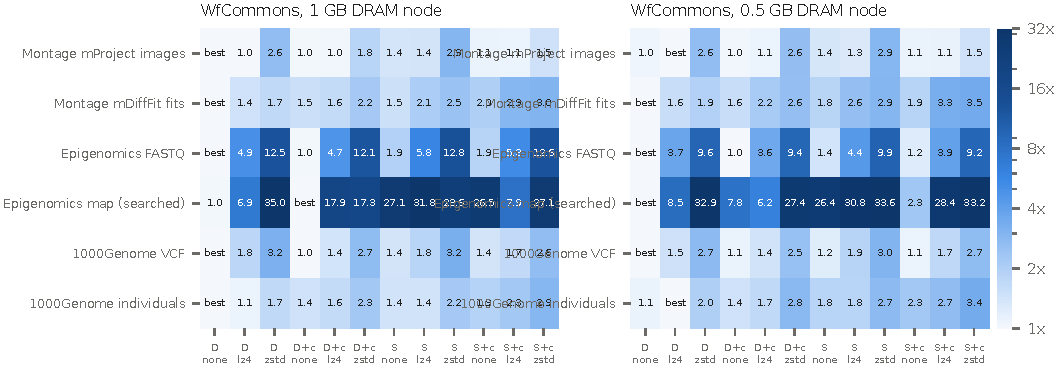
\includegraphics[width=\textwidth]{figures/fig_motivation.pdf}
\caption{Time of each valid composition relative to the best one for each WfCommons phase (median
of 3 runs). Columns: placement (D = DRAM-first, S = SSD-first), +c = cache, codec; the indexer is
set as each phase requires. ``lost'' = writes refused because the window did not fit.}
\label{fig:motivation}
\end{figure*}

\begin{table}[t]
\caption{Best composition per WfCommons phase (placement/cache/codec) and how much slower the worst
valid composition is.}
\label{tab:best}
\small\resizebox{\columnwidth}{!}{\IfFileExists{tables/best_wf.tex}{\begin{tabular}{lrrrr}
\toprule
Phase & \multicolumn{2}{c}{1 GB DRAM} & \multicolumn{2}{c}{0.5 GB DRAM} \\
 & best & worst/best & best & worst/best \\
\midrule
Montage mProject images & DRAM/--/none & 2.9$\times$ & DRAM/--/lz4 & 2.9$\times$ \\
Montage mDiffFit fits & DRAM/--/none & 3.0$\times$ & DRAM/--/none & 3.5$\times$ \\
Epigenomics FASTQ & DRAM/--/none & 12.8$\times$ & DRAM/--/none & 9.9$\times$ \\
Epigenomics map (searched) & DRAM/cache/none & 35.0$\times$ & DRAM/--/none & 33.6$\times$ \\
1000Genome VCF & DRAM/--/none & 3.2$\times$ & DRAM/--/none & 3.0$\times$ \\
1000Genome individuals & DRAM/--/none & 2.9$\times$ & DRAM/--/lz4 & 3.4$\times$ \\
Cycles season output & pending &  & pending &  \\
SoyKB realigned BAMs & pending &  & pending &  \\
SoyKB gVCFs (searched) & pending &  & pending &  \\
Seismology SAC traces & pending &  & pending &  \\
SRAsearch reads & pending &  & pending &  \\
\bottomrule
\end{tabular}
}{\pending{best-stack table}}}
\end{table}

\section{The Storage System Context}\label{sec:ssc}
The SSC is the text the model reads before each decision. Its design follows five rules, fixed
before any evaluation run and motivated by known failure modes of small models (they copy what
they see, ignore negation, and are weak with raw numbers):
\begin{enumerate}
\item \textbf{No module prose.} Options appear only as answer choices; nothing describes what a
  module ``usually'' costs. Prose encodes general knowledge, which is what is wrong on a given node.
\item \textbf{Positive, typed facts.} Feasibility is a fact per option (``lz4: fits in the free
  space''), never a negation or advice.
\item \textbf{Digested numbers.} Measured costs are turned into words: \emph{fastest}, \emph{a
  little slower}, \emph{about $N\times$ slower}.
\item \textbf{Experience from this node only.} For each option, the evidence is a
  similarity-weighted summary over the $k=3$ most similar \emph{other} workloads measured on this
  node. The current workload is never in its own memory, so the context cannot contain the answer.
  Similarity uses block size, writes and reads per window, and compressibility.
\item \textbf{Speed and feasibility are separate.} A neighbour on which an option lost writes
  (because it did not fit) is left out of that option's speed estimate; feasibility for the current
  window is stated separately.
\end{enumerate}

Figure~\ref{fig:ssc} shows the SSC for one Epigenomics alignment window, generated from the
measured grid of the evaluation node. The window declares that it is searched later, so the
indexer question states that it is required. The three most similar other workloads measured on
the node say that DRAM is fastest (SSD about 5$\times$ slower), that the cache helps (about
2$\times$), and that no compression is fastest. The best measured composition for this phase is
exactly DRAM, cache, indexer, no compression.

The same evidence protects against general knowledge. For a 1000Genome VCF window (compressibility
21$\times$), the compression question states that all three options fit and that, on similar
workloads on this node, no compression is fastest and lz4 about 2$\times$ slower. Without the SSC,
the model compresses it (\S\ref{sec:modules}).

\begin{figure}[t]
\begin{lstlisting}
## NODE EXPERIENCE (other workloads measured on this node)
workload A (similarity: low): 256 blobs of 4 MB, write-only, 1.4x
workload B (similarity: low): 256 blobs of 4 MB, write-only, 1.0x
workload C (similarity: low): 1024 blobs of 4 MB, write-only, 6.4x
## CURRENT WINDOW
writes: 660 blobs of 512 KB; 660 reads (1 per blob); 2.0x
data written per window: 0.32 GB; free space: 3.0 GB
searched later: yes; latency critical: no

Which storage tier should the data be placed on?
- dram: on similar workloads on this node: fastest
- ssd:  on similar workloads on this node: about 5x slower
Should the cache be in the chain?
- enable:  on similar workloads on this node: fastest
- disable: on similar workloads on this node: about 2x slower
Which compression setting should the chain use?
- none: fits; on similar workloads on this node: fastest
- lz4:  fits; on similar workloads on this node: about 2x slower
- zstd: fits; on similar workloads on this node: about 6x slower
Should the indexer track the window?
- enable:  required: the data is searched later
- disable: the data is not searchable later
\end{lstlisting}
\caption{The SSC for an Epigenomics alignment window on the 1\,GB node (abridged; generated from the
measured grid). The model answers DRAM, cache, indexer, no compression: the measured best.}
\label{fig:ssc}
\end{figure}

\section{\sys{} Design}\label{sec:design}
\paragraph{Default chain.} No module is on by default. A chain starts as the core alone (DRAM-first,
no cache, no indexer, no compression); modules are added only when a decision asks for them.

\begin{figure*}[t]
\centering
\resizebox{0.95\textwidth}{!}{% System overview (TikZ). \input from main.tex.
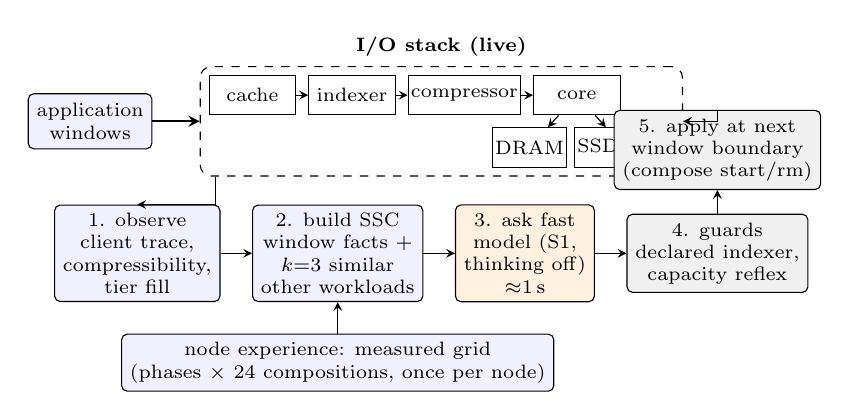
\begin{tikzpicture}[
  font=\scriptsize, >=stealth, node distance=4mm,
  box/.style={draw, rounded corners=2pt, align=center, inner sep=3pt, minimum height=7mm},
  data/.style={box, fill=blue!6}, model/.style={box, fill=orange!12}, det/.style={box, fill=gray!12},
  mod/.style={draw, fill=white, minimum width=11mm, minimum height=5mm, inner sep=1pt}]
  % composable I/O chain
  \node[mod] (cache) {cache};
  \node[mod, right=1.5mm of cache] (idx) {indexer};
  \node[mod, right=1.5mm of idx] (cmp) {compressor};
  \node[mod, right=1.5mm of cmp] (core) {core};
  \node[mod, below=1.5mm of core, xshift=-6mm, minimum width=8mm] (dram) {DRAM};
  \node[mod, below=1.5mm of core, xshift=6mm, minimum width=8mm] (ssd) {SSD/PFS};
  \draw[->] (cache) -- (idx); \draw[->] (idx) -- (cmp); \draw[->] (cmp) -- (core);
  \draw[->] (core) -- (dram); \draw[->] (core) -- (ssd);
  \node[draw, dashed, rounded corners, fit=(cache)(core)(dram)(ssd), inner sep=3pt,
        label={[font=\scriptsize\bfseries]above:I/O stack (live)}] (chain) {};
  \node[data, left=6mm of chain] (app) {application\\windows};
  \draw[->, thick] (app) -- (chain);
  % loop
  \node[data, below=7mm of app, xshift=6mm] (obs) {1. observe\\client trace,\\compressibility,\\tier fill};
  \node[data, right=of obs] (ssc) {2. build SSC\\window facts +\\$k$=3 similar\\other workloads};
  \node[model, right=of ssc] (llm) {3. ask fast\\model (S1,\\thinking off)\\$\approx$1\,s};
  \node[det, right=of llm] (guard) {4. guards\\declared indexer,\\capacity reflex};
  \node[det, above=of guard, yshift=-1mm] (act) {5. apply at next\\window boundary\\(compose start/rm)};
  \node[data, below=4mm of ssc] (grid) {node experience: measured grid\\(phases $\times$ 24 compositions, once per node)};
  \draw[->] (chain.south west) ++(2mm,0) |- (obs.north);
  \draw[->] (obs) -- (ssc); \draw[->] (ssc) -- (llm); \draw[->] (llm) -- (guard); \draw[->] (guard) -- (act);
  \draw[->] (act.north) |- (chain.east);
  \draw[->] (grid) -- (ssc);
\end{tikzpicture}
}
\caption{\sys{} overview. Once per workload window, the client trace and the node's measured
experience become the SSC; a fast model answers four typed questions; two deterministic guards
check the answer; the new chain is applied to the live runtime at the next window boundary.}
\label{fig:overview}
\end{figure*}

\paragraph{The decision loop.} \sys{} runs while the workload runs, once per window
(Figure~\ref{fig:overview}):
\begin{enumerate}
\item \textbf{Observe.} When a window ends, summarize its client trace (writes and reads, block
  size, reads per write), sample the compressibility of one blob, and read the tier fill levels.
\item \textbf{Build the SSC.} Find the three most similar other workloads in the node's experience
  and write one evidence line per option (Figure~\ref{fig:ssc}). Building the SSC takes milliseconds.
\item \textbf{Ask.} Send four typed questions (placement, cache, indexer, compression) to the fast
  model with thinking off; it returns one JSON object with one option per question (constrained
  decoding, temperature 0).
\item \textbf{Guard.} Two deterministic guards wrap the model: a \emph{declared-requirement gate}
  (data declared as searched later always gets the indexer) and a \emph{capacity reflex} (a window
  that would not fit uncompressed is compressed; during a window, a watermark at 40\% free space
  adds the strongest codec live). Every controller in the evaluation, including the rules, runs
  with the same guards.
\item \textbf{Apply.} The new chain takes effect at the next window boundary. Module changes add or
  remove pools on the running runtime (median 0.2\,s); a
  placement change restarts it. A canary put/get verifies every new chain.
\end{enumerate}

\paragraph{Asynchronous decisions.} In blocking mode the workload waits for the answer. In
asynchronous mode the workload keeps running and the answer is applied at the first window
boundary after it arrives. A 1\,s answer is then hidden behind the next window's I/O; a 45\,s answer
from a reasoning model arrives many windows late and acts on stale context.

\paragraph{Node experience.} The per-option evidence comes from a measured grid: every workload
phase in the node's memory under every composition. On the evaluation node this took 1--2 hours per
node setup (24 compositions $\times$ 7 phases $\times$ 3 repeats, more when the second tier is slow). It is measured once per node,
before the workload runs; everything else happens online. \S\ref{sec:ablation} measures what a node
with no experience (a cold start) loses.

\section{Implementation}\label{sec:impl}
\sys{} runs on the IOWarp composable runtime~\cite{iowarp}. Two changes made single-node
composition meaningful there.
\paragraph{Cache.} The runtime's cache is a cross-node read cache: the node that owns a blob keeps no copy.
On one node every blob is owner-local, so the cache was a pass-through and its on/off decision was
noise. We added an opt-in single-node mode (populate on read miss, delete on write; coherent because
a single node has no foreign writers) and mark the SSD tier durable so cache copies stay in DRAM.

\paragraph{Replication.} Same-node replicas were placed by score only, so with two equal disks the
copy landed on the same disk as the original. We added device anti-affinity: devices that already
hold a copy are tried last.

Both changes pass the runtime's own cache, replication, indexer and compressor test suites (17 of 17 tests).

\section{Evaluation}\label{sec:eval}
\subsection{Setup}\label{sec:setup}
\paragraph{Platform.} One NCSA Delta node (AMD EPYC 7763, 64 cores, 256 GB RAM, local NVMe, 4
NVIDIA A100-40GB), allocated exclusively so no other job shares it. The storage runtime and the
workload run on cores 0--31; each model runs in its own Ollama server on one A100, pinned to cores
32--63. Three node setups: \emph{1\,GB}: 1\,GB DRAM tier + 2\,GB NVMe tier; \emph{0.5\,GB}: 0.5\,GB
DRAM + 1.5\,GB NVMe; \emph{DRAM+PFS}: 0.5\,GB DRAM + a 2\,GB tier on the Lustre parallel file system.

\paragraph{Workload: a WfCommons campaign.} Seven scientific workflows from the WfInstances
traces~\cite{wfcommons} (Pegasus on Chameleon) share the node, as on an allocation that runs a
campaign of workflows. Each contributes its dominant I/O stages as phases (Table~\ref{tab:phases}):
Montage reprojected images (4\,MB, 10.4 readers per file) and plane fits (1\,KB); Epigenomics split
FASTQ (6\,MB) and alignments (512\,KB, searched later); 1000Genome chromosome VCF (2\,GB per window,
21$\times$ compressible) and per-individual results (28\,KB, already compressed); Cycles crop-season
outputs (304\,KB, rarely re-read); SoyKB realigned BAMs (80\,KB, 10 readers per file) and per-sample
gVCFs (43\,KB, searched later); Seismology receiver functions (4.6\,KB SAC files); and SRAsearch
downloaded reads (1.5\,GB per window). File sizes and reuse are the traces'; counts are scaled so a
window is a meaningful amount of I/O; contents are synthesized in each format (FITS, FASTQ, alignment
text, VCF, Cycles tables, SAC, compressed BAM), since the traces record sizes only. A schedule is a
random sequence of 9 blocks of 3--5 windows, each block one phase; the phases want different stacks
(\S\ref{sec:motivation}), so no fixed stack fits a schedule.

\paragraph{Leave-one-workflow-out experience.} The SSC's node experience is the measured grid of the
\emph{other} workflows: when \sys{} decides for a phase of SoyKB, no SoyKB phase is in its experience.
Every workflow is therefore new to the SSC when it runs, while the hand-tuned fixed stack is chosen
with the measured grid of the very windows it is scored on.

\paragraph{Controllers.} \emph{Fixed stacks (what runs today):} the default stack as shipped;
the default with the indexer on for streams the user declared searchable; and the best single stack
for the scenario, chosen with the measured grid of the very windows it is scored on (an expert who
hand-tuned the configuration with hindsight). \emph{\sys{}:} S1 + SSC with qwen3-4B and llama3.1-8B,
thinking off. \emph{Alternative deciders} (design justification): S2, qwen3-4B with thinking on and no
SSC; the same fast models without the SSC (only the option list) and with an SSC without node
experience; hand-written expert rules (written once, before any run) and a variant that picks the
codec by capacity; a model-free lookup that takes the option with the best SSC evidence; online
exploration (no model, no SSC): explore-first (try each valid stack once per phase, then keep the
fastest), UCB1, and $\epsilon$-greedy from the default stack, fresh per run, and explore-first that
keeps what it learned across the 10 test schedules (a site that has run the campaign before). The
explorers observe one measured repeat per window (real measurement noise), are told the phase identity
for free, and have the same guards. For live runs, an oracle knows each window's best stack in
advance. Model sizes 1.7B--14B appear in the size sweep.

\paragraph{Metrics.} \emph{Accuracy}: the share of decisions whose composition is within 25\% of
the best measured one for that window (the median repeat-to-repeat spread of the grid is 4--10\%).
\emph{Slowdown}: geometric mean over windows of the chosen composition's time over the best one's.
Lost writes or a broken declared requirement count as the worst valid composition. \emph{Decision
time}: model latency per window. \emph{End-to-end time} (live): I/O + recomposition + blocking
decision time. Confidence intervals resample whole schedules (seeds), since windows of one schedule
are not independent.

\paragraph{Protocol.} The SSC design (v12, \S\ref{sec:ssc}) was fixed on practice schedules of
synthetic simulation-output phases, which are not part of the evaluation, before any run of the
WfCommons campaign; no constant was tuned on the campaign. Offline replays use 10 schedules per node
setup (seeds 101--110, 36--41 windows each); live runs use schedules 301--303. Every grid cell is the
median of 3 repeats, each starting from empty tiers, on an exclusively allocated node.

\subsection{Main result: automatic composition vs.\ fixed stacks}\label{sec:main}
Figure~\ref{fig:main} and Table~\ref{tab:main} compare \sys{} with fixed I/O stacks and with the
alternative deciders on the WfCommons campaign.

\begin{figure*}[t]
\centering
\IfFileExists{figures/fig_main_accuracy_speed.pdf}{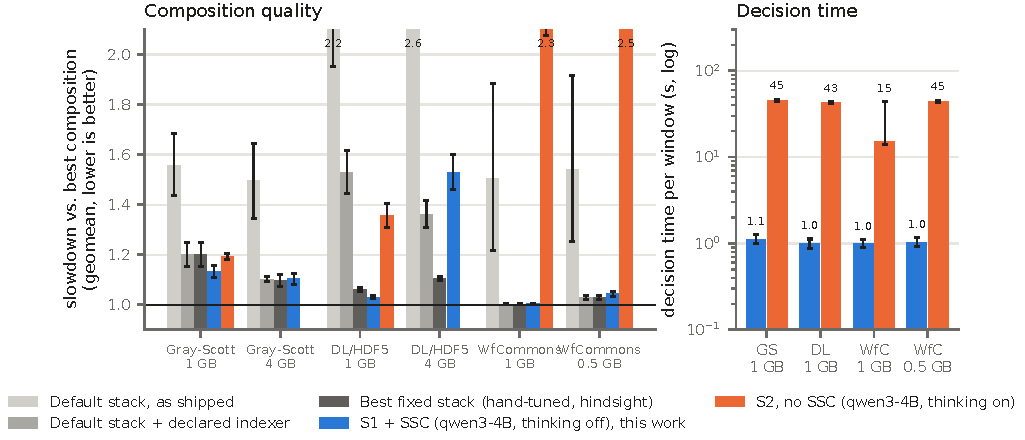
\includegraphics[width=0.95\textwidth]{figures/fig_main_accuracy_speed.pdf}}{\pending{fig main accuracy speed}}
\caption{Left: slowdown of each controller's compositions vs.\ the best measured composition per
window (geometric mean over 10 schedules; 95\% CI over schedules). Gray: fixed stacks, from the
default as shipped to the best stack chosen with hindsight; blue: \sys{}; orange: a reasoning model
without the SSC. Right: decision time per window (median, IQR).}
\label{fig:main}
\end{figure*}

\begin{table*}[t]
\caption{Offline replay of the WfCommons campaign, 10 schedules per node setup: accuracy (\% of
decisions within 25\% of the best) and slowdown vs.\ the best composition (geometric mean).
$^\dagger$ fewer than 10 schedules.}
\label{tab:main}
\small\resizebox{\textwidth}{!}{\begin{tabular}{l}
\toprule
 &  \\
Controller &  \\
\midrule
\multicolumn{1}{l}{\emph{Fixed I/O stacks (today)}} \\
\midrule
\multicolumn{1}{l}{\emph{Automatic composition (this work)}} \\
\midrule
\multicolumn{1}{l}{\emph{Alternative deciders (design justification)}} \\
\bottomrule
\end{tabular}
}
\end{table*}

\textbf{\sys{} vs.\ fixed stacks.} \pending{slowdown of \sys{} vs.\ the default as shipped, the
default with the declared indexer, and the hand-tuned stack, per node setup; how far each fixed stack
is from the best, and which phases make it so.}

\textbf{Offline tuners, STELLAR included, are bounded by the hand-tuned stack.} An offline tuner
such as STELLAR~\cite{stellar} profiles the target application, tries configurations in reruns of it,
and outputs one configuration for the next run. However well it searches, its result is a fixed stack,
and the best fixed stack for a campaign is the hand-tuned stack we report, chosen with the measured
grid of the very windows it is scored on, i.e.\ with more information than any tuner gets from a
profiling run and five trials. Its slowdown is therefore a lower bound on what any offline tuner can
reach on this campaign, at a cost of at least one profiling run and several full reruns of the target,
which \sys{} does not need; where the campaign's phases want different stacks, \sys{} can beat the bound
because it changes the stack within the run \pending{(margin over the bound per node setup)}. We do not
reimplement STELLAR itself: it tunes Lustre parameters, not stack composition, and its design (a
frontier model with retrieval over manuals, Darshan analysis and trial runs) would have to be
reinterpreted to choose modules; the bound holds for any such reinterpretation.

\textbf{Where \sys{} loses.} \pending{phases where \sys{} is worse than a fixed stack, and why
(which evidence was missing from the other workflows).}

\textbf{Why a fast model with the SSC, and not a reasoning model or rules.} \pending{S1 without the
SSC; S2 without the SSC (accuracy, slowdown, 15--45\,s per decision); expert rules and the capacity
variant; the model-free lookup.}

\textbf{Why not learn the stack online?} \pending{explore-first / UCB1 / $\epsilon$-greedy per run, and
exploration kept across runs, vs.\ \sys{}.} With 24 stacks per phase and phases of 3--5 windows, an
explorer that starts fresh cannot finish exploring before a phase ends; one that keeps what it learned
across runs of the same campaign eventually measures the target directly, which the SSC never does.
The two are complementary: the SSC gives a new workflow a good stack from its first window, and
recording each observed window as experience would let \sys{} converge like the learner on recurring
campaigns (\S\ref{sec:limits}). Exploration cost grows with the number of compositions, the SSC's
per-option evidence does not (\S\ref{sec:bigger}).

\textbf{What the model adds.} The accuracy comes from the SSC, not from the model: a lookup that takes
the best-evidenced option is as good where the evidence is decisive. The model earns its place where
the evidence ranking misleads \pending{(cases from the campaign)}, and v12 therefore lets decisive
evidence decide and asks the model only on near-ties. It also combines typed facts of different kinds
(fit, declared intent, measured cost, whether the window moved) without hand-written combination
rules, which the lookup needs for each new fact, and it makes a new module or question a matter of
adding evidence lines, not code. A small model with thinking off is enough for this role; a larger or
reasoning model is not better (Table~\ref{tab:sweep}).

\subsection{Live end-to-end runs}\label{sec:live}
\begin{table}[t]
\caption{Live runs of the WfCommons campaign, 1\,GB node: mean per schedule (schedules 301--303).}
\label{tab:live}
\small\resizebox{\columnwidth}{!}{\IfFileExists{tables/live_1g_wf.tex}{\input{tables/live_1g_wf.tex}}{\pending{live table}}}
\end{table}

Table~\ref{tab:live} and Figure~\ref{fig:live} show live runs, in which each controller drives the
storage runtime through a schedule of the campaign. \pending{end-to-end time of the default stack,
the hand-tuned stack, \sys{} blocking and asynchronous, the rules, S1 without the SSC, the oracle,
and S2 blocking and asynchronous; decision and recomposition time.}

\begin{figure}[t]
\centering
\IfFileExists{figures/fig_live_1g_wf.pdf}{\includegraphics[width=\columnwidth]{figures/fig_live_1g_wf.pdf}}{\pending{live figure}}
\caption{Live runs of the WfCommons campaign, 1\,GB node: time per schedule split into I/O,
recomposition and blocking decision time.}
\label{fig:live}
\end{figure}

\subsection{Which modules are used, and why}\label{sec:modules}
Table~\ref{tab:modules} lists, per phase, the measured best chain and the chain each controller
chose most often (with its accuracy in that phase). \pending{per module: where \sys{} enables the
cache (re-read phases: Montage images, SoyKB BAMs), the indexer (alignments, gVCFs), compression
(windows that would not fit, or a slow second tier), and where it leaves each off, with the evidence
that decided it.} Without the SSC, the same model enables every module for every phase.

\begin{table}[t]
\caption{Per phase: measured best chain and the most frequent chain each controller chose (share of
its decisions within 25\% of the best), 1\,GB node.}
\label{tab:modules}
\small\resizebox{\columnwidth}{!}{\IfFileExists{tables/modules_1g_wf.tex}{\input{tables/modules_1g_wf.tex}}{\pending{modules table}}}
\end{table}

\subsection{What each part contributes}\label{sec:ablation}
\pending{Option list only; SSC without node experience (a new node); full SSC with the guards off;
guards only.}

\subsection{Model size}
\begin{table}[t]
\caption{Model size, WfCommons campaign, 1\,GB node (thinking off).}
\label{tab:sweep}
\small\resizebox{\columnwidth}{!}{\IfFileExists{tables/sweep_wf.tex}{\input{tables/sweep_wf.tex}}{\pending{sweep table}}}
\end{table}
\pending{qwen3-1.7B, 4B, 8B, 14B and llama3.1-8B with and without the SSC.}

\subsection{What the SSC costs: how much must a node measure?}\label{sec:lc}
The SSC's evidence comes from a grid measured once per node setup: every composition on each measured
phase, 3 repeats. Figure~\ref{fig:lc} asks how much of it is needed: we restrict the node experience
to random subsets of $N$ of the 11 phases ($N=2,4,6,8$; the same subsets for every node setup), keep
leaving the decided workflow out, and score the decisions on the full grid. \pending{accuracy vs.\
$N$ for the lookup and \sys{}; measurement minutes for the smallest $N$ that reaches full accuracy.}

\begin{figure*}[t]
\centering
\IfFileExists{figures/fig_learning_curve.pdf}{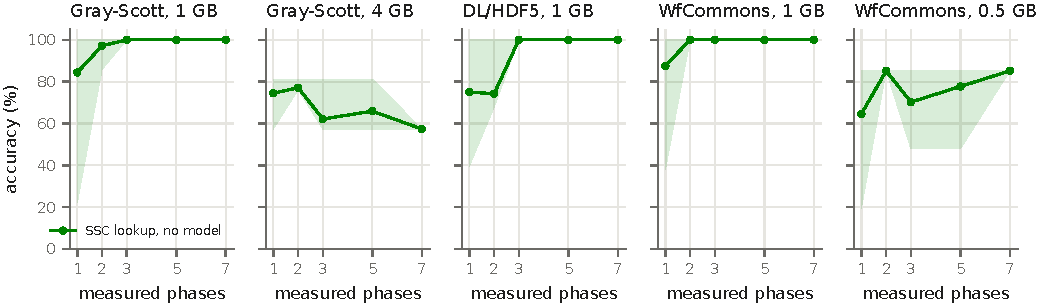
\includegraphics[width=\textwidth]{figures/fig_learning_curve.pdf}}{\pending{fig learning curve}}
\caption{Accuracy vs.\ the number of phases the node has measured (its experience; the decided
workflow is always left out); line: mean over random subsets, band: min--max.}
\label{fig:lc}
\end{figure*}

\subsection{Portability across node setups}\label{sec:portability}
For each node setup, the experience is re-measured and the same SSC code rebuilds the context; the
expert rules stay as written. \pending{0.5\,GB: which phases change stack when DRAM halves.
DRAM+PFS: spilling to the parallel file system is expensive, so compression and the cache pay off where
they did not on NVMe (the 1000Genome VCF is 5$\times$ slower with the default stack there); how
\sys{}, the fixed stacks and the rules follow.}

\subsection{Sensitivity}
\paragraph{Measurement noise.} \pending{rescoring every key arm with each single repeat of the grid in
place of the median.}
\paragraph{Accuracy threshold.} \pending{orders of the main arms at 10\%, 25\%, 50\% and 2$\times$.}
\paragraph{What is fixed by design.} The SSC has a small number of constants, all set before any
evaluation run: the word bins of the evidence (fastest up to 1.15$\times$, a little slower up to
1.6$\times$), the decisive-evidence threshold (every other option more than 1.15$\times$ slower), and
$k=3$ similar workloads.

\begin{table}[t]
\caption{The WfCommons campaign's phases: source trace stage, blob size, blobs and reads per window,
compressibility, and declared intent.}
\label{tab:phases}
\small\resizebox{\columnwidth}{!}{\IfFileExists{tables/phases_wf.tex}{\begin{tabular}{llrrrl}
\toprule
Phase & trace stage & blob & blobs & reads & searched \\
\midrule
Montage mProject images & mProject & 4\,MB & 180 & 1872 & no \\
Montage mDiffFit fits & mDiffFit & 1\,KB & 4230 & 4230 & no \\
Epigenomics FASTQ & fastqSplit/filterContams & 6\,MB & 165 & 165 & no \\
Epigenomics map (searched) & map & 512\,KB & 660 & 660 & yes \\
1000Genome VCF & ALL.chrN.250000.vcf & 4\,MB & 512 & 512 & no \\
1000Genome individuals & individuals & 28\,KB & 2600 & 3900 & no \\
Cycles season output & cycles/fertilizer\_increase & 304\,KB & 1600 & 640 & no \\
SoyKB realigned BAMs & indel\_realign & 80\,KB & 1000 & 10000 & no \\
SoyKB gVCFs (searched) & haplotype\_caller & 43\,KB & 2000 & 4000 & yes \\
Seismology SAC traces & sG1IterDecon & 4.5\,KB & 4000 & 4000 & no \\
SRAsearch reads & fasterq-dump & 8\,MB & 192 & 192 & no \\
\bottomrule
\end{tabular}
}{\pending{phases table}}}
\end{table}

\section{Discussion: Bigger Stacks}\label{sec:bigger}
Our stacks have four decisions and 24 compositions. The runtime we use already offers more: ten
codecs including the error-bounded lossy SZ3 and ZFP, replication, write-back and write-through
persistence, a shared-memory write-through cache, and a third tier (DRAM, NVMe and the parallel file
system). With three placements, cache, indexer, eight codecs, replication and two persistence modes,
a stack has $3\cdot2\cdot2\cdot8\cdot2\cdot2=384$ compositions. That growth hurts each alternative
differently. A hand-tuned fixed stack needs the target workload measured under all 384; online
exploration needs at least 384 windows per phase before it can exploit, far longer than a phase. The
SSC asks one question per decision and needs, per option, its cost on similar workloads with the other
decisions at their best; such evidence can be measured by varying one decision at a time from the best
of the others, so the measurement grows with the sum of the option counts (19) rather than their
product. Lossy codecs add a decision only the application can bound (the error tolerance), which fits
the SSC's declared-intent facts. We leave the larger stacks to future work.

\section{Related Work}
\paragraph{LLM-based storage and system tuning.} STELLAR~\cite{stellar} reproduces an I/O expert's
tuning workflow for Lustre with a large model, retrieval over manuals, Darshan analysis and a growing
rule set, and reaches near-optimal settings within five reruns of the application.
ELMo-Tune-V2~\cite{elmotune} and StorageXTuner~\cite{storagextuner} tune key-value and storage
engines, and GPTuner~\cite{gptuner}, LLMTune~\cite{llmtune} and $\lambda$-Tune~\cite{lambdatune}
tune database knobs. All tune parameters of a fixed system \emph{between} runs, with the target
workload's trace and trial runs, and produce one static configuration. \sys{} changes the composition
of the stack \emph{within} a run, per window, for a workload it has not measured, with a small local
model. Any such tuner's output is a fixed stack, so the hand-tuned stack chosen with hindsight in
\S\ref{sec:main} bounds what it can reach on our campaign. STELLAR-style tuning of each module's
parameters is complementary to choosing the modules. IOAgent~\cite{ioagent} and
ION~\cite{ion} use LLMs to diagnose I/O behavior from traces rather than to act on it.
\paragraph{Classical I/O autotuning.} Model-based and search-based autotuners for HDF5, MPI-IO and
parallel file systems~\cite{behzadauto,h5tuner}, reinforcement learning (CAPES~\cite{capes}) and
Bayesian optimization~\cite{bayesio,sapphire} tune numeric knobs of a fixed stack over hundreds to
thousands of runs. Online tuners adjust parameters that can change at run time, such as Lustre client
RPC and cache settings (DIAL~\cite{dial}, CARAT~\cite{carat}) or I/O library settings
(SCTuner~\cite{sctuner}); they tune knobs of one layer, not which layers are in the path.
\paragraph{Learned placement and compression.} Sibyl~\cite{sibyl}, Harmonia~\cite{harmonia} and the
Adaptive Storage Learner~\cite{asl} learn data placement across tiers; HCompress~\cite{hcompress} and
online SZ/ZFP selection~\cite{szzfp} choose a compressor. Each makes one kind of decision; \sys{}
decides placement, cache, indexer and codec together, and from evidence measured on other workloads
rather than from training on the target.
\paragraph{Composable storage.} Mochi~\cite{mochi}, ADIOS2~\cite{adios2}, HDF5 VOL~\cite{hdf5vol},
Hermes~\cite{hermes}, IOFlow~\cite{ioflow} and Crystal~\cite{crystal} provide composition and
policy mechanisms whose policies are written by people; \sys{} is a chooser for such mechanisms.
\paragraph{Fast and slow models.} Dual-process systems~\cite{sofai,fastslow}, model
cascades~\cite{frugalgpt,routellm} and two-time-scale controllers~\cite{symbiotic} keep slow models
out of the fast loop; NetLLM~\cite{netllm} shows single-pass models meet control-loop latency. \sys{}
shows that with grounded context the fast model alone is accurate enough.
\paragraph{Workflow benchmarks.} WfCommons~\cite{wfcommons} provides execution traces and
generators of scientific workflows; we use its traces to derive realistic I/O phases.

\section{Limitations}\label{sec:limits}
\emph{Transfer needs similar evidence.} The SSC can only state what a measured workload shows; when
no other workflow behaves like the decided one on some decision, the evidence for that decision is
misleading \pending{(campaign cases)}. Measuring a more diverse set of workflows per node, or recording each
observed window as new experience, would close such gaps. \emph{Scope.} One node type and single-node
composition; four decisions (replication and prefetching are not yet decisions); the workflow file
contents are synthesized in the real formats, since the traces record sizes only. \emph{Cold start.} The
SSC needs a measured grid per node setup \pending{(time)}; on a node with no measurements the SSC is no
better than no context \pending{(campaign numbers)}.
\emph{Declared intent.} Part of the gain over the default stack comes from indexing streams the user
declared searchable, which a configuration could also do; we report the default with and without it.

\section{Conclusion}
HPC applications still run on fixed I/O stacks, even where composable storage could give every
workload its own. \sys{} composes the stack automatically and online: a fast model
with thinking off, given a context built from the node's own measurements of other workloads, chooses
a composition per window in about a second, \pending{X}$\times$ faster than the default stack and
\pending{compared with} a stack hand-tuned with hindsight, without measuring the target workflow.
A reasoning model is too slow to act at phase granularity, and without node evidence it is not more
accurate; a few measured workloads per node are enough to give a small model that evidence.

\bibliographystyle{ACM-Reference-Format}
\bibliography{refs}
\end{document}
